%\documentclass{beamer}
\documentclass[xcolor=pdftex,dvipsnames,table]{beamer}
\usepackage{verbatim}
\usepackage{amsmath}

\usetheme{Luebeck}
\usecolortheme[named=RawSienna]{structure}
\setbeamerfont{frametitle}{family=\rmfamily,shape=\itshape}
%\setbeamertemplate{frametitle}[default][center]
\defbeamertemplate*{title page}{customized}[1][]
{
  \vspace{1.9cm}

% Content
  \begin{minipage}{10cm}

  % Title and subtitle
  \begin{beamercolorbox}[center,#1]{title}
    \vskip0.04em%
    \usebeamerfont{title}\inserttitle\par%
    \ifx\insertsubtitle\@empty%
    \else%
      \vskip0.3em%
      {\usebeamerfont*{subtitle}\usebeamercolor*[fg]{subtitle}\insertsubtitle\par}%
    \fi%
    \vskip0.3em%
  \end{beamercolorbox}%

  \vskip1em\par

  % Display author(s)
  \begin{beamercolorbox}[center,#1]{author}
    \usebeamerfont{author}\insertauthor{}
  \end{beamercolorbox}

  \vskip1em\par

  % Institute
  \begin{beamercolorbox}[center,#1]{institute}
    \usebeamerfont{institute}\insertinstitute{}
  \end{beamercolorbox}

  \vskip1em%

  % Date
  \begin{beamercolorbox}[center,#1]{date}
    \usebeamerfont{date}\insertdate
  \end{beamercolorbox}\vskip0.5em

  \end{minipage}
  \hspace{0.6cm}
  \vfill

  \begin{flushleft}
  {\usebeamercolor[fg]{titlegraphic}\inserttitlegraphic\par}
  \end{flushleft}
  \hfill

%  \usebeamerfont{title}\inserttitle\par
%  \usebeamerfont{subtitle}\usebeamercolor[fg]{subtitle}\insertsubtitle\par
%  \bigskip
%  \usebeamerfont{author}\insertauthor\par
%  \usebeamerfont{institute}\insertinstitute\par
%  \usebeamerfont{date}\insertdate\par
%  \usebeamercolor[fg]{titlegraphic}\inserttitlegraphic
}

\title{The Rubik's Cube and Group Theory}
\subtitle{"In mathematics you don’t understand things. You just get used to them." - J. von Neumann}
\author{David Buchmann}
\institute{Cisco Systems}

\date{\today}

\begin{document}

\maketitle

\section{Rubik's Cube Background}
\begin{frame}
  \frametitle{Kubik Rubik}
  \begin{columns}[cc]
    \column{2.5in}
    \begin{itemize}
    \item Erno Rubik (a Hungarian professor of Interior Design) created the Rubik's cube in 1974.
    \item 100,000,000 cubes have been sold worldwide.
    \item There are 26 visible cubies on the 3 by 3 Rubik's cube (8 corner cubies, 12 edge cubies, and 6 center cubies)
    \item God's number: Every Rubik's cube can be solved in 20 or less moves.
  \end{itemize}
    \column{0.5in}
    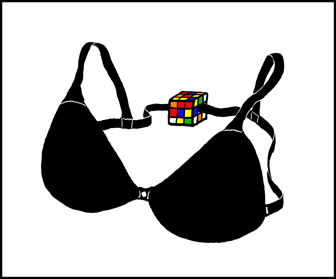
\includegraphics[scale=0.33]{rubik_frustration.png}
  \end{columns}
\end{frame}

\section{Group Theory}
\subsection{Groups}
\begin{frame}
  A group is a mathematical construct consisting of a set and an operation satisfying the following axioms:
  \begin{itemize}
    \item Associativity - operation must satisfy $(a + b) + c = a + (b + c)$
    \item Closure - applying the operation on any combination of elements in the set must yield another element inside the set.
    \item Inverse element - Every element in the set must have an inverse element
    \item Identity element - An element which is it's own inverse
  \end{itemize}
\end{frame}

\begin{frame}
  Example: The hours on a 12-hour clock forms a group $G$ under addition (and is denoted $ \mathbb{Z} / 12\mathbb{Z}$ or $\mathbb{Z}_{12}$ for short)
  \begin{itemize}
    \item 0 is the identity element
    \item Set \{0,1,2,3,4,5,6,7,8,9,10,11\} has 12 elements ($|G| = 12$)
    \item Operation is + modulo 12
  \end{itemize}
  
\end{frame}

\subsection{Subgroups}
\begin{frame}
  \begin{itemize}
    \item A subgroup of a group is a construct using the same operation, but a subset of the elements that will still maintain the group axioms.
    \item Example: every 4th hour on a 12-hour clock
    \item Operation is + modulo 12
    \item Set \{0, 4, 8, 12 \}
  \end{itemize}
\end{frame}

\subsection{Abelian Groups}
\begin{frame}
  Here for completeness, feel free to zone out for this slide.
  \begin{itemize}
    \item A commutative ($a * b = b * a, a, b \in G$) group is known as an Abelian group.
    \item Abelian groups can be generated from one member of the group (written $G = \{ a^n, n \in \{0, 1, \hdots \}$).
    \item A subgroup of a non-commutative group may be Abelian.
  \end{itemize}
\end{frame}

\subsection{Permutation Groups}

\begin{frame}
  \begin{itemize}
    \item A permutation group is a group where the elements are permutations, and the operation is composition.
    \item The symmetric group $S_n$ is the group of permutation of n elements.
    \item Cayley's Theorem: (Zone out now!) Any group $G$ where $|G|=n$ is isomorphic to a subgroup of $S_n$.
  \end{itemize}
\end{frame}

\begin{frame}
  Even and odd permutations
  \begin{itemize}
    \item We can write permutations in cycle notation. 
    \item $(123)(45)$ means move 1 to 2, 2 to 3, 3 to 1, 4 to 5, and 5 to 4.
    \item Every permutation can be written as a cycle, and every cycle of length n can be written as a product of (n-1) 2-cycles.
    \item $(123) = (12)(13)$
    \item The product of an even number of 2-cycles is known as an even permutation, and an odd number is known as an odd permutation.
    \item Order: Writing a permutation like this tells us how many times it needs to be applied to get to an unpermuted state (the order), e.g. (123) must be applied 3 times
  \end{itemize}
\end{frame}

\section{The Rubik's Group}
\subsection{The Rubik's Group}
\begin{frame}
  \frametitle{The Rubik's Group}
  \begin{itemize}
    \item The group representing the Rubik's cube ($ \mathbf{R} $) is a group where the elements are all possible permutations of the Rubik's cube, and the operation is concatenation of these permutations.
    \item The Rubik's group is not Abelian: e.g. $FU != UF$
    \item Every permutation in the Rubik's group is an even permutation.
  \end{itemize}
\end{frame}

\subsection{Even Permutations}
\begin{frame}
  \begin{itemize}
    \item Any face turn will permute 8 elements (4 edges, and 4 vertices). Naming them 1 to 4 and A to D we get: $(1234)(ABCD) = (12)(13)(14)(AB)(AC)(AD)$, which is an even permutation
    \item Any combination of $n$ even permutations is even.
    \item Thus, all permutations of the rubik's cube are even permutations
  \end{itemize}
\end{frame}

\section{Solving the Rubik's cube}

\subsection{Subgroups}
\begin{frame}
  \begin{itemize}
    \item The concepts behind solving the Rubik's cube all involve splitting the solution of the Rubik's group into subgroups.
    \item For this talk we consider a very simple algorithm often used for blind solving.
    \item The algorithm splits solving into four steps. Each step in the solve only changes cubies in the subgroup related to that step
      \begin{itemize}
      \item Edge permutation (Subgroup permuting edges while maintaining orientation)
      \item Corner permutation (Subgroup permuting corners while maintaining orientation)
      \item Edge orientation (Subgroup orienting edges while maintaining permutation)
      \item Corner orientation (Subgroup orienting corners while maintaining permutation)
      \end{itemize}
    \item The cube is solved
  \end{itemize}
\end{frame}

\subsection{Permute edges}
\begin{frame}
  \begin{itemize}
  \item Not all face turns are valid when permuting edges (which follows from the idea that this is a subgroup).
  \item Allowed turns: 
  \item Algorithm to permute three edges:
  \item
  \end{itemize}
\end{frame}
\end{document}
